\documentclass[12pt,notes=show]{beamer} % pour l'impression, tout n'apparait qu'une fois \documentclass[handout,12pt]{beamer}
\usepackage[utf8x]{inputenc}
\usepackage{ucs}
\usepackage[french]{babel}
\usepackage{todonotes}
\usepackage{tikz}

%pour le theme
%\usetheme{CambridgeUS}

%\usetheme{Goettingen}
\useinnertheme{}
\setbeamertemplate{blocks}[rounded][shadow=true]
\setbeamercolor{block title}{bg=blue!20}
\setbeamercolor{block title alerted}{bg=blue!20} 
\setbeamercolor{block title example}{bg=blue!20}

%Mettre la section courante en titre de diapo (pour champ de titre non-vide)
\addtobeamertemplate{frametitle}{\frametitle{\insertsubsectionhead}}{}

\author{Alice \textsc{Dinsenmeyer} \& Thomas \textsc{Lechat} \\ encadré par Olivier Richoux}

\title{ Modes localisés dans les structures périodiques}
\subtitle{M1 Acoustique}
\date{\today}



\begin{document}

\begin{frame}
	\titlepage
\end{frame}
\begin{frame}
\tableofcontents
\end{frame}

\section{Introduction}
\begin{frame}{~}
\insertsectionhead
\begin{itemize}
\item But du projet: Mettre en évidence expérimentalement un mode localisé
\item Contexte: Méta-matériaux, applications à l'acoustique non-linéaire
\end{itemize}
	\centering
	\begin{figure}
		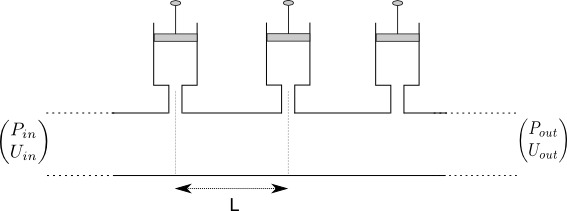
\includegraphics[scale=0.35]{schema_reseau_infini.png}\hfill
		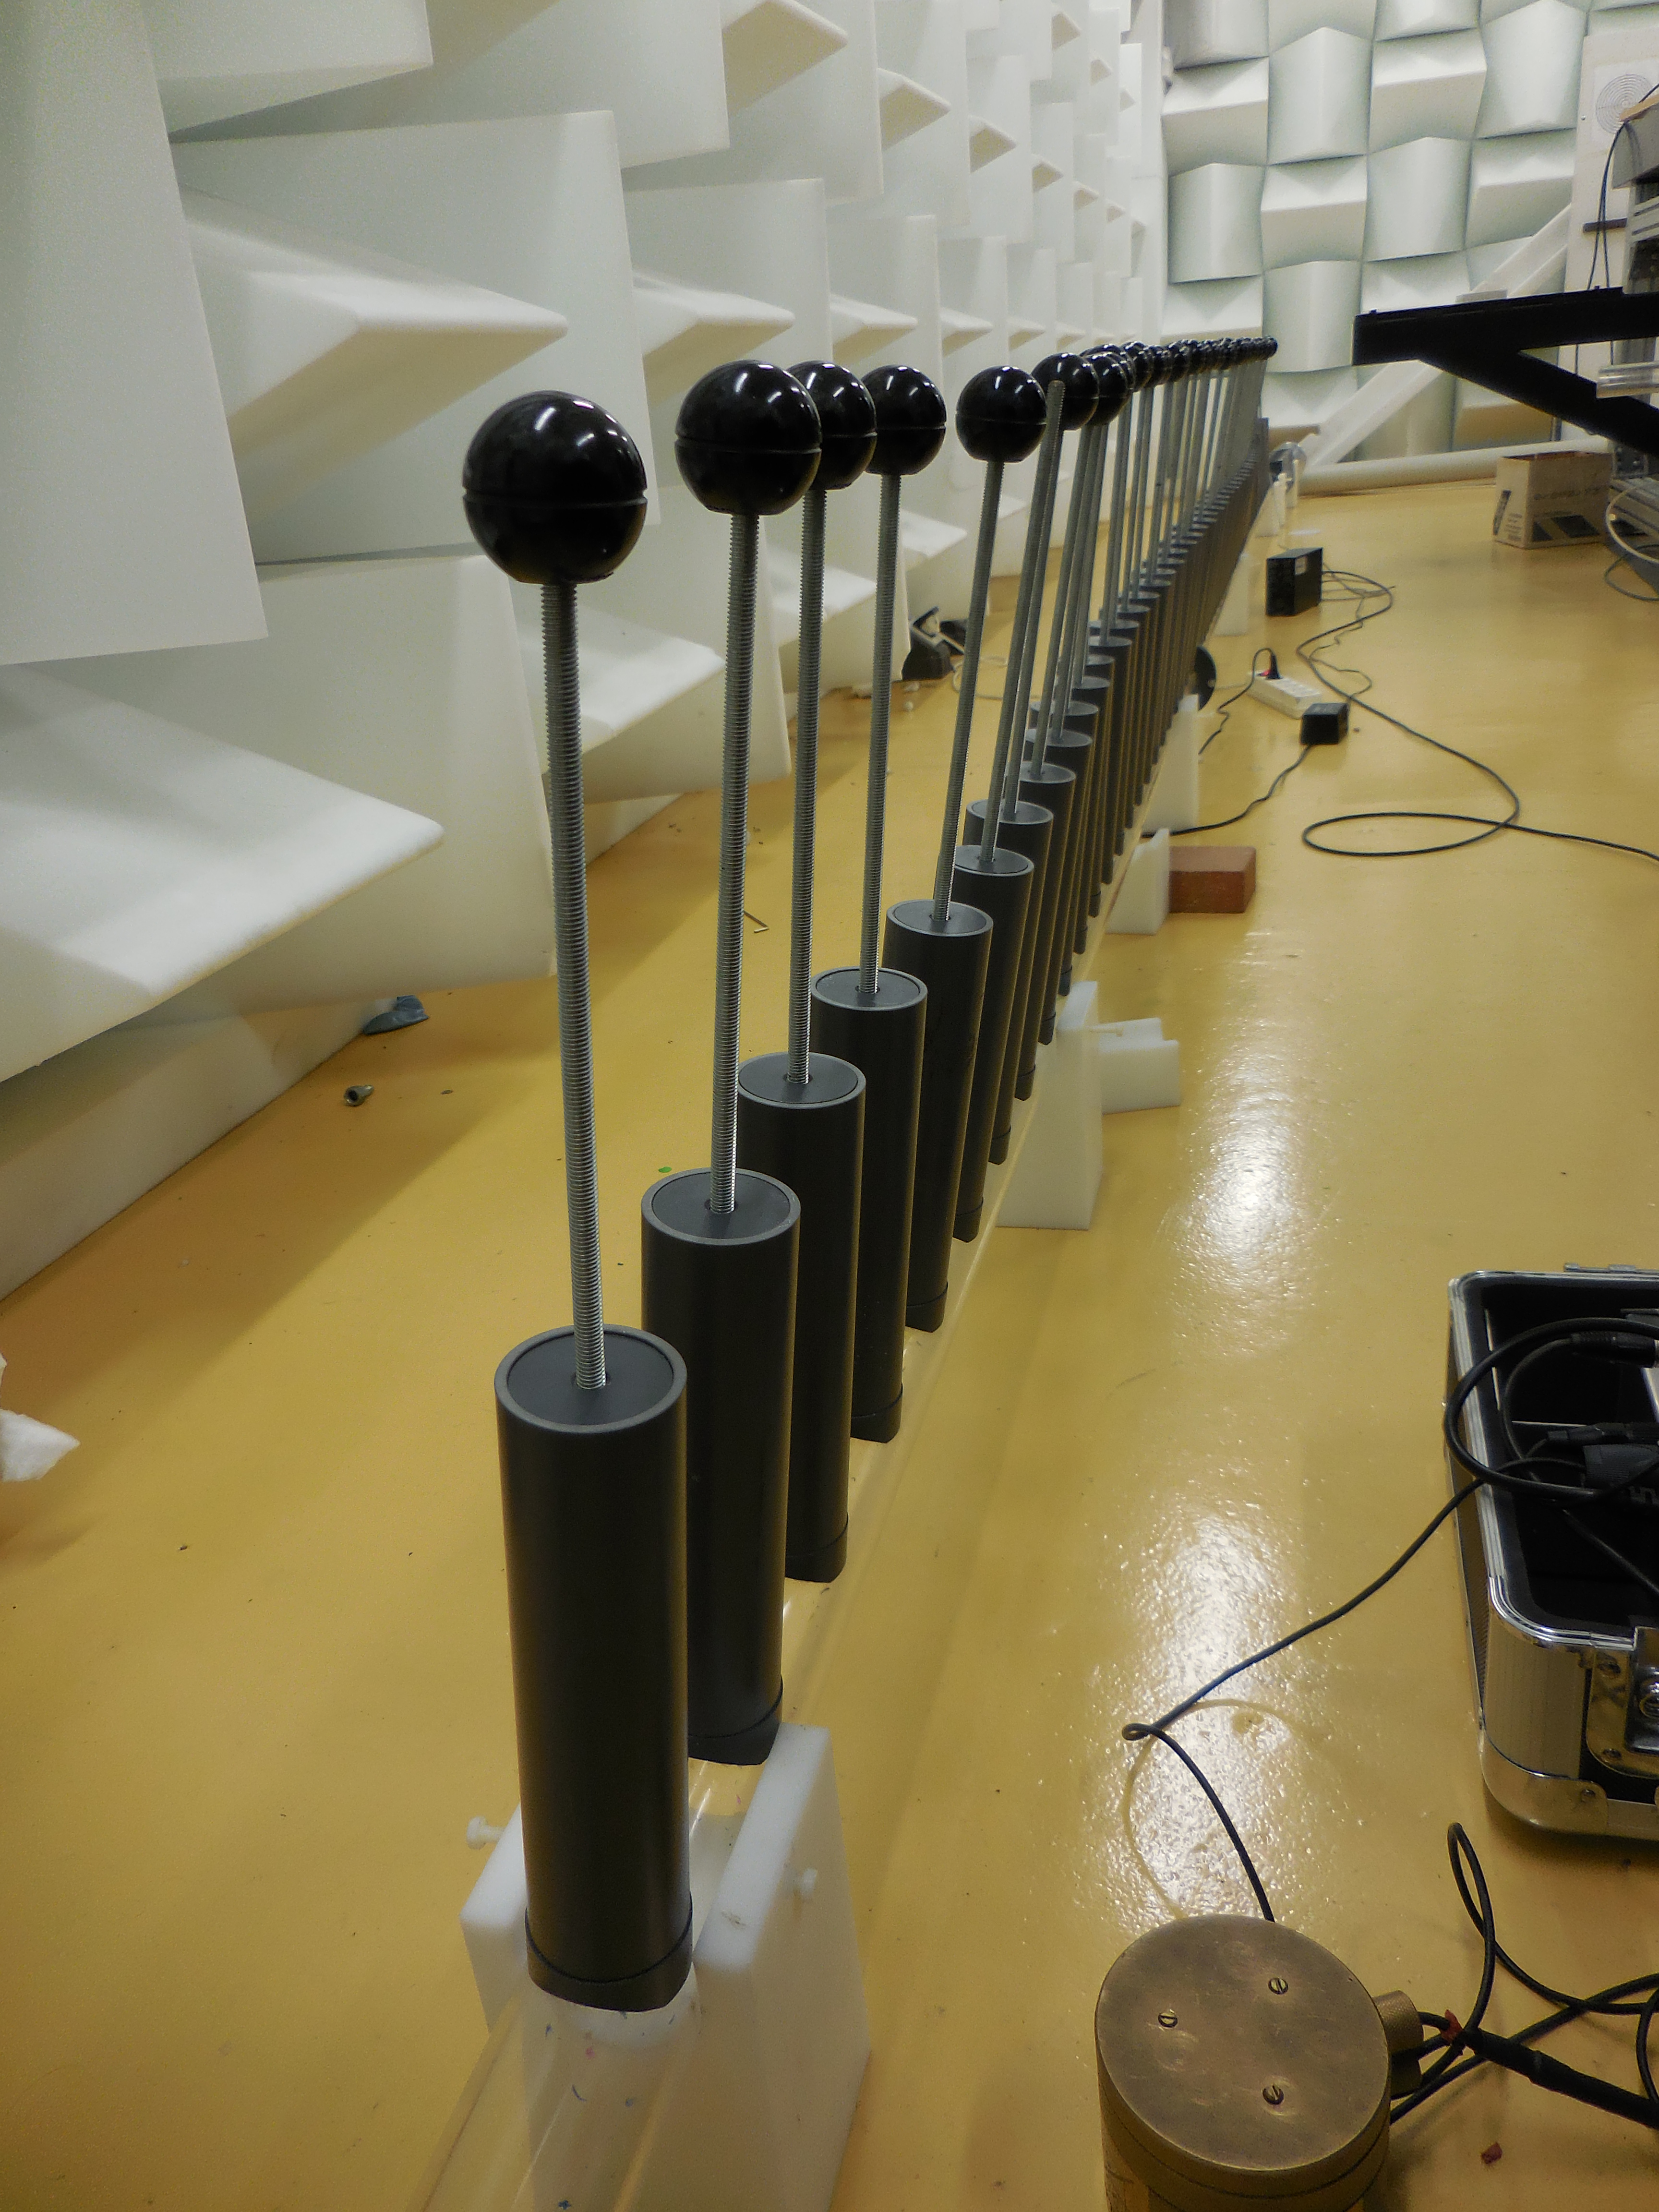
\includegraphics[scale=0.02]{photo.jpg}
	\end{figure}
	
Réseau de résonateurs branchés en dérivation sur un guide d'onde. La terminaison est anéchoïque.
	
\end{frame}


\section{Réseau infini}

\subsection{Formalisme matriciel}
\begin{frame}{~}
\begingroup \tiny
\begin{block}{Une matrice de guide:}
		\centering
	\begin{eqnarray*}
	\begin{pmatrix} p(x_1) \\ v(x_1) \end{pmatrix} = \begin{pmatrix} \cosh(kL) & \frac{j\omega\rho}{k} \sinh(k L) \\  \frac{k}{j\omega\rho}\sinh(k L) & \cosh(k L) 		\end{pmatrix} 	\begin{pmatrix} p(x_2) \\ v(x_2) \end{pmatrix}
	\end{eqnarray*}
\end{block}


\begin{block}{Une matrice de résonateur:}
\centering
\begin{eqnarray*}
\begin{pmatrix} P_e \\U_e \end{pmatrix}&=&\begin{pmatrix} \cos(k L_n) & j Z_{n} \sin(k L_n) \\ \frac{1}{Z_{n}} \sin(k L_n) & \cos(k L_n) \end{pmatrix} \begin{pmatrix} \cos(k L_c) & j Z_{c} \sin(k L_c) \\ \frac{1}{Z_{c}} \sin(k L_c) & \cos(k L_c) \end{pmatrix} \begin{pmatrix} P_s \\ 0  \end{pmatrix} \\
\begin{pmatrix} P_e \\U_e \end{pmatrix}&=&\begin{pmatrix} r_1 & r_2 \\ r_3 & r_4 \end{pmatrix} \begin{pmatrix} P_1 \\ 0  \end{pmatrix} 
\end{eqnarray*}
\end{block}
\endgroup

La multiplication des 2 permet de décrire un réseau infini composé des 2 éléments.
\end{frame}




\begin{frame}{~}
Ajout des pertes viscothermiques: changement sur $k$ et $Z_c$
\begin{eqnarray*}
 k =  \frac{\omega}{c_0} \left( 1 + \frac{\beta}{s}(1+(\gamma-1)/ \chi \right) \\
 Z_c =  \frac{\rho c_0}{S} \left( 1 + \frac{\beta}{s}(1-(\gamma-1)/ \chi \right) 
\end{eqnarray*}

Dans ces expressions, on a:
\begin{itemize}
 \item  $s=R/ \delta$ avec $\delta = \sqrt{\frac{2 \mu}{\rho \omega}}$
 \item  $\chi = \sqrt{P_r}$ ou $P_r$ est le nombre de Prandtl
 \item $\beta = (1-j)/\sqrt{2}$ 
 \item $\mu$ la viscosité de l'air
\end{itemize}
\end{frame}


\subsection{Bande interdites}
\begin{frame}{~}
	\vspace{0.5cm}
Des bandes interdites sont crée par la périodicité du réseau et à cause des résonateurs.	
	\begin{figure}
		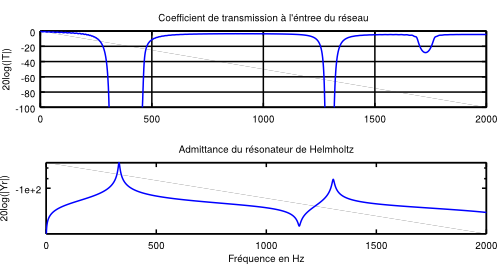
\includegraphics[scale=0.45]{transmission.png}
	\end{figure}
	\vspace{-1cm}
	
	\begin{columns}
		
		\column{0.3 \textwidth}
		\flushright
		\begin{tikzpicture}
			\draw[line width=1pt,black!70,->] (0.2,0) --  (0,-0.7);
 		\end{tikzpicture}\\ \centering
 		...liée à la résonance du résonateur de Helmholtz
		
		\column{0.3 \textwidth}
		\flushright
		\begin{tikzpicture}
			\draw[line width=1pt,black!70,->] (0.3,0) --  (0,-0.7);
 		\end{tikzpicture}\\ \centering
 		...liée à la résonance de la cavité du résonateur
 		
 		\column{0.3 \textwidth}
 		\centering
 		\begin{tikzpicture}
			\draw[line width=1pt,black!70,<-] (0,0) -- + (0,0.7);
 		\end{tikzpicture}\\
 		...liée à la périodicité (bande de Bragg)
		
	\end{columns}
\end{frame}


\section{Ajout d'une singularité}
\begin{frame}{~}
\insertsectionhead
	En ajoutant une \textbf{singularité} sur un des résonateurs\\
	  \hspace{1cm} $\hookrightarrow$ création d'un mode localisé \\

	\vspace{1cm}
	\begin{block}{Problématique}
		\begin{itemize}
			\item Où placer cette singularité ?
			\item Comment choisir sa fréquence de résonance ?
			\item Comment l'observer expérimentalement ?
		\end{itemize}
	\end{block}
 
\end{frame}

\subsection{Influence de la position et de la fréquence de résonance du défaut}
\begin{frame}{~}
\begin{itemize}
\item Si la fréquence du défaut est en dehors d'une bande interdite, il agit comme un mur et l'onde ne ce propage pas au delà. 
\item Sinon on à alors une localisation de l'onde dans le réseau.
\end{itemize}

Dans le second cas, afin de voir apparaître le mode sur les coefficients de transmissions et réflexions, celui-ci doit se trouver au début du réseau ou que le réseau ai peut d’éléments.
\end{frame}


\subsection{Simulation de la pression dans le tube}
\begin{frame}{~}
La pression dans le tube est simulé grâce au formalise matriciel en partant d'une sortie anéchoïque.
\begin{figure}
\centering
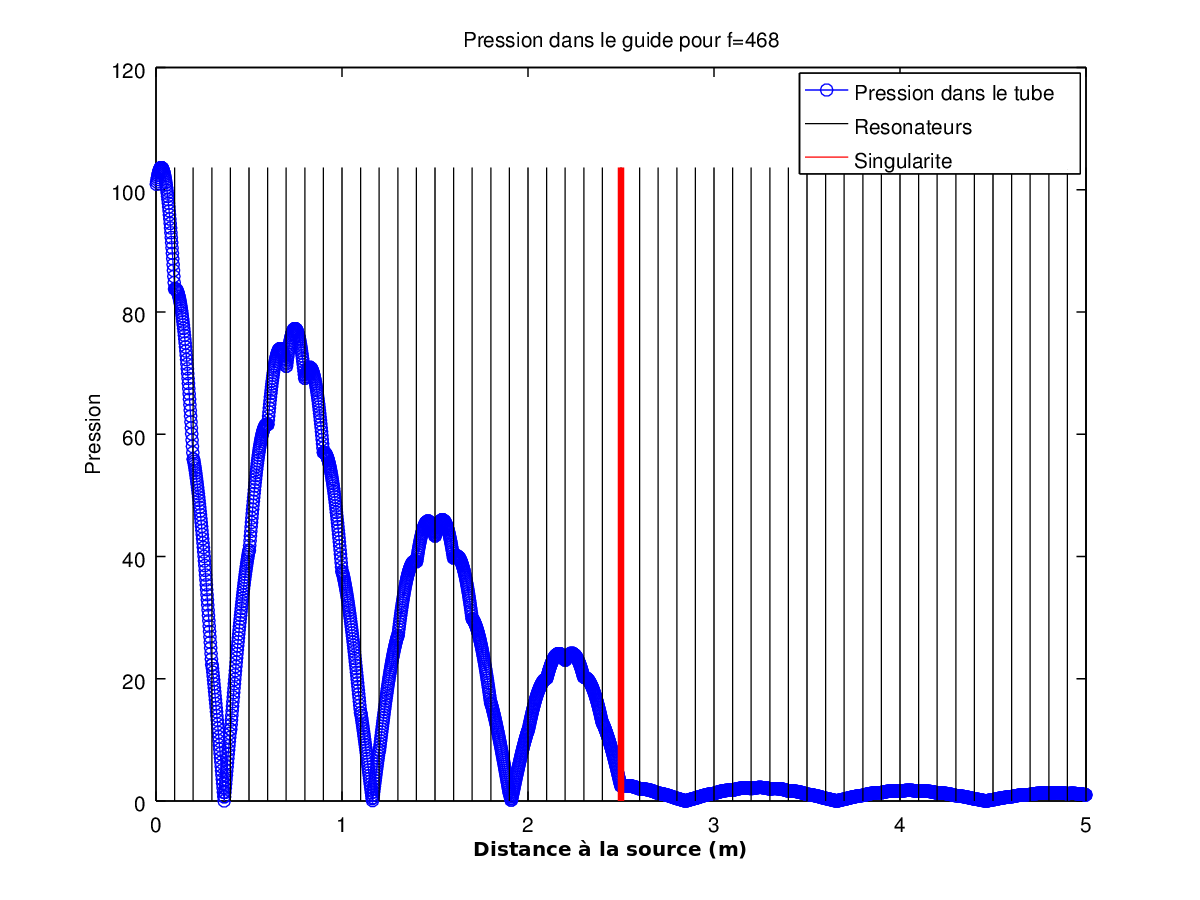
\includegraphics[scale=0.1]{visu_pression_defavo.png} \hfill
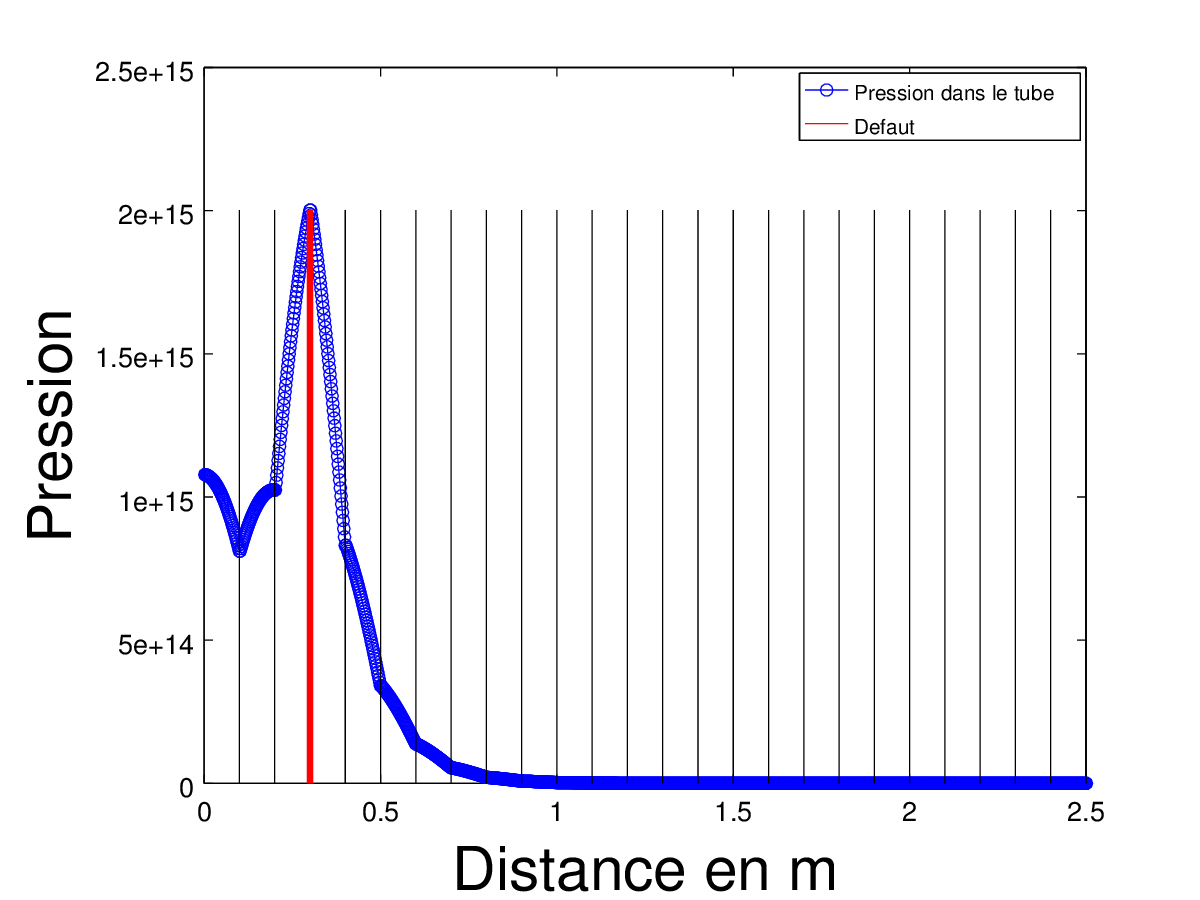
\includegraphics[scale=0.1]{visu_pression_favo2.png}
\end{figure}
\end{frame}


\subsection{Changements sur les coefficients de réflexion et transmission}
\begin{frame}{~}
Dans une bonne configuration (un réseau de petite taille ou avec un défaut au début du réseau), on peut voir un pic émerger sur la transmission et la réflexion.

%\begin{itemize}
%\item Un capteur d'impédance à une extrémité du réseau permet de calculer le coefficient de réflexion et de transmission.
%\item L'insertion d'un capteur dans le banc de mesure permet la mesure d'un mode localisé.
%\end{itemize}

\begin{figure}
\centering
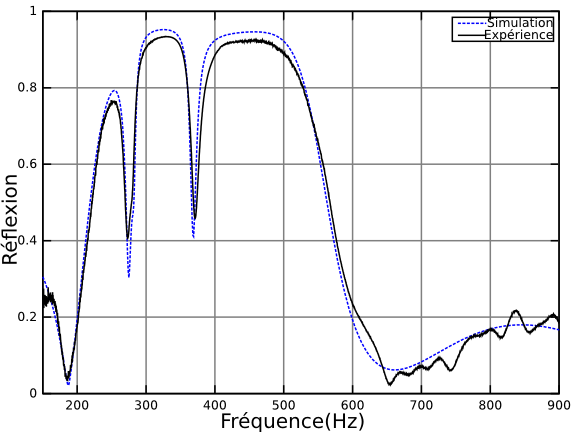
\includegraphics[scale=0.2]{R_5HR165_8cm_pos3.png}\hfill
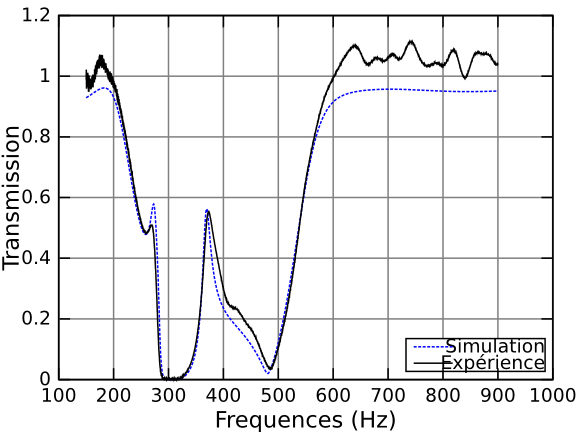
\includegraphics[scale=0.2]{T_5HR165_8cm_pos3.png}
\caption{ {\small Réseau de 5 cellules avec une longueur de cavités de $16~cm$ pour les résonateurs et $8~cm$ pour le défaut. Celui-ci se trouve en 3\textsuperscript{ème} position dans le réseau.}}
\end{figure}

\end{frame}

\section{Visualisation expérimentale du mode localisé}


\subsection{Mesure de la pression dans le tube}
\begin{frame}{~}
Un microphone est ensuite inséré dans le réseau pour mesurer la pression en tout point de celui-ci.
\begin{figure}
\centering
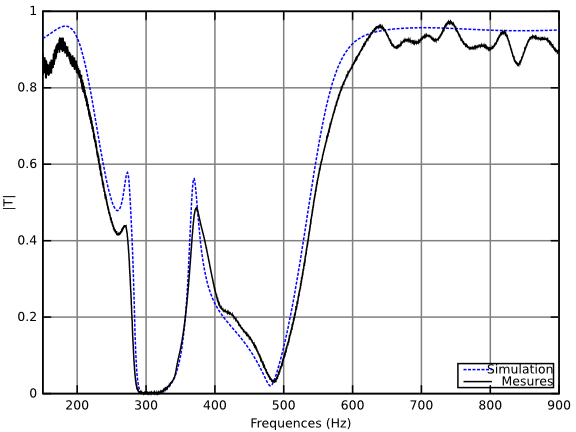
\includegraphics[scale=0.23]{bim.png}\hfill
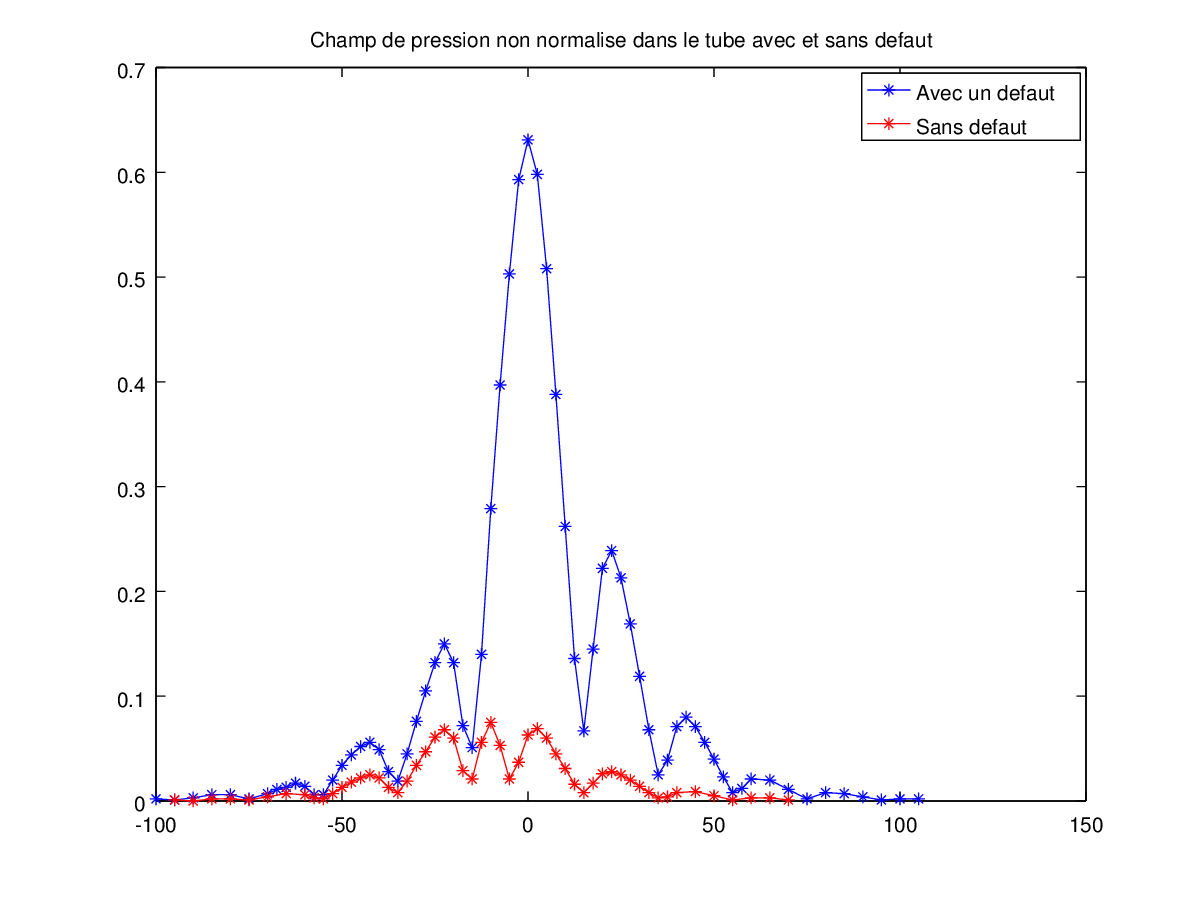
\includegraphics[scale=0.2]{non_norm_lin.png}
\end{figure}

On a bien une localisation de la pression avec un fort niveau dans le réseau.
Mais, problème de protocole de mesure: le réseau n'est plus symétrique a cause de la source.
\end{frame}


\subsection{Changement de géométrie du réseau}
\begin{frame}{~}
Ajout d'un 2\textsuperscript{ème} résonateur comme défaut avec source au centre pour retrouver un système symétrique.

\begin{figure}
\centering
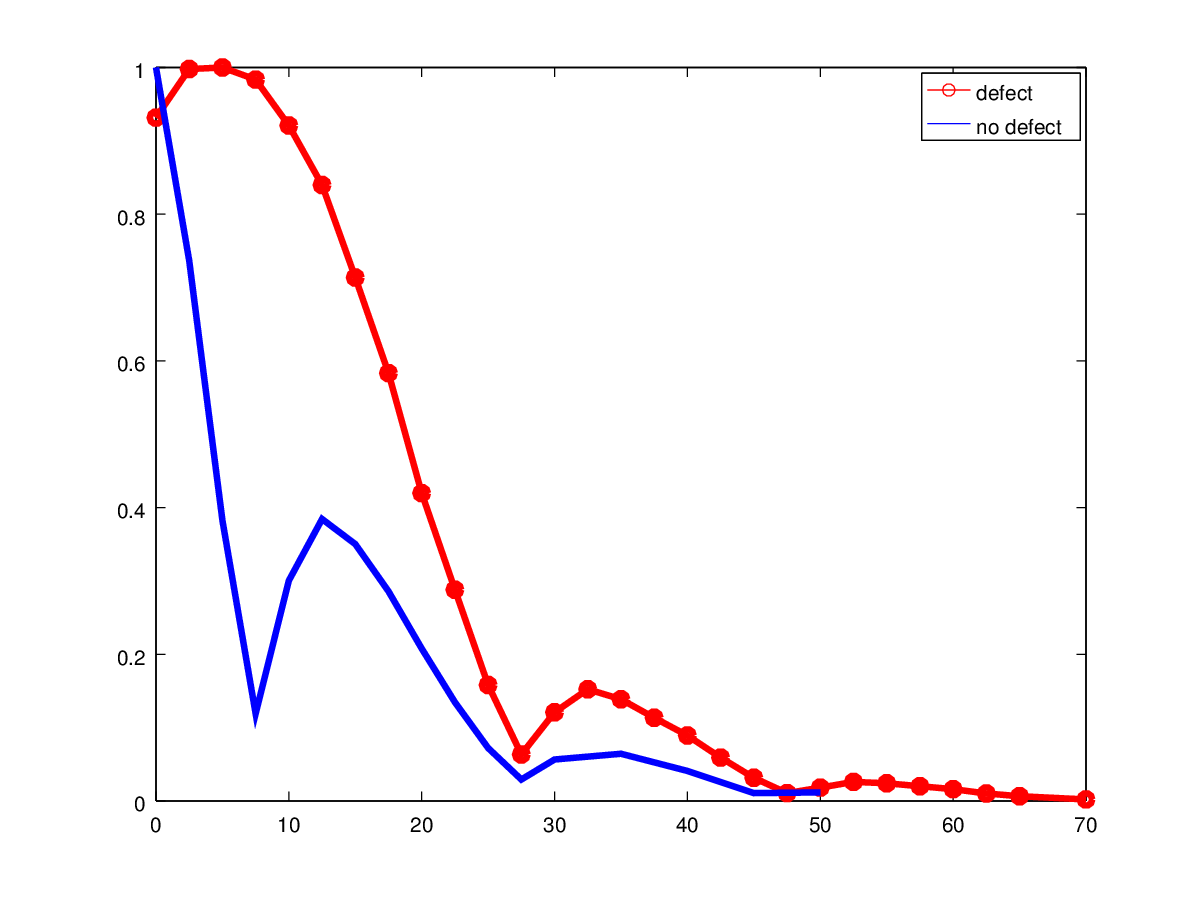
\includegraphics[scale=0.2]{comparaison_decroissance_lin.png}\hfill
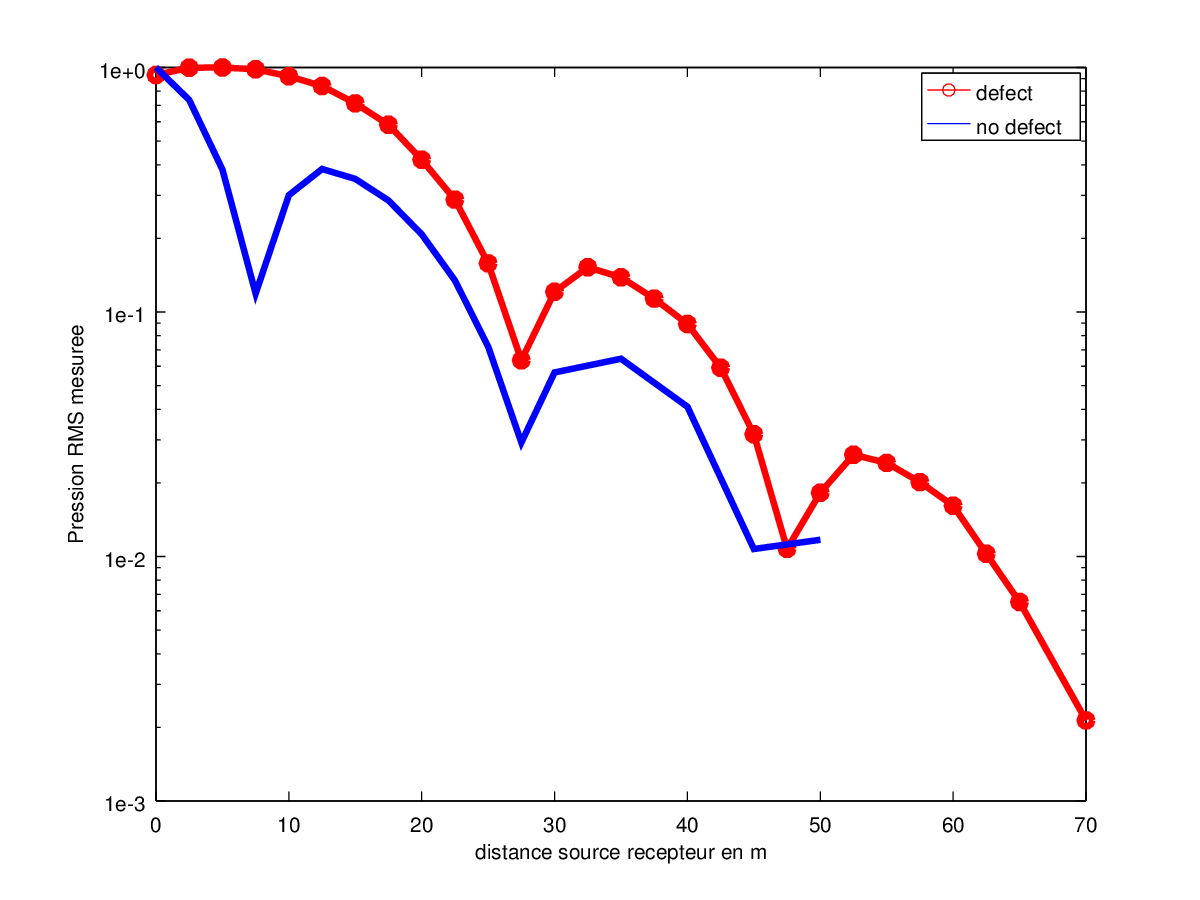
\includegraphics[scale=0.2]{comparaison_decroissance_log.png}
\end{figure}

Même décroissance dans les 2 cas. Celle-ci correspond à la partie imaginaire de la constante de propagation dans le réseau. 
Le modèle théorique est cependant différent.

\end{frame}

\section{Conclusions}
\begin{frame}{~}
\insertsectionhead
	\begin{block}{Notions abordées}
		\centering
		\begin{itemize}
			\item Acoustique non-linéaire : dispersion
			\item Réseaux acoustiques
			\item Modes localisés
		\end{itemize}
	\end{block}
	
	\begin{exampleblock}{Savoir-faire acquis}
		\begin{itemize}
			\item Formalisme matriciel
			\item Simulations numériques
			\item Mesures de transmission
		\end{itemize}
	\end{exampleblock}
	
	\begin{alertblock}{Outils utilisés}
		\begin{itemize}
			\item Git
			\item Octave
			\item Capteur d'impédance CTTM
		\end{itemize}
	\end{alertblock}
	
\end{frame}


\end{document}